\documentclass[12pt, a4paper, twoside]{book}
\usepackage[utf8]{inputenc}
\usepackage{hyperref}
\usepackage{graphicx}
\usepackage{subfig}
\usepackage{eso-pic}
\usepackage{wrapfig}
\usepackage{lineno}
\usepackage{tikz}
\usetikzlibrary{shapes.geometric, arrows}
\linenumbers

\tikzstyle{arrow} = [thick,->,>=stealth]
\tikzstyle{startstop} = [rectangle, rounded corners, minimum width=3cm, minimum height=1cm,text centered, draw=black, fill=red!30]
\tikzstyle{process} = [rectangle, minimum width=3cm, minimum height=1cm, text centered, draw=black, fill=orange!30]
\tikzstyle{decision} = [diamond, minimum width=3cm, minimum height=1cm, text centered, draw=black, fill=green!30]


\newcommand\AlCentroPagina[1]{%
\AddToShipoutPicture*{\AtPageCenter{%
\makebox(0,0){\includegraphics%
[width=1.3\paperwidth]{#1}}}}}

\makeatletter
% Une commande sembleble à \rlap ou \llap, mais centrant son argument
\def\clap#1{\hbox to 0pt{\hss #1\hss}}%
% Une commande centrant son contenu (à utiliser en mode vertical)
\def\ligne#1{%
  \hbox to \hsize{%
    \vbox{\centering #1}}}%
% Une comande qui met son premier argument à gauche, le second au 
% milieu et le dernier à droite, la première ligne ce chacune de ces
% trois boites coïncidant
\def\haut#1#2#3{%
  \hbox to \hsize{%
    \rlap{\vtop{\raggedright #1}}%
    \hss
    \clap{\vtop{\centering #2}}%
    \hss
    \llap{\vtop{\raggedleft #3}}}}%
% Idem, mais cette fois-ci, c'est la dernière ligne
\def\bas#1#2#3{%
  \hbox to \hsize{%
    \rlap{\vbox{\raggedright #1}}%
    \hss
    \clap{\vbox{\centering #2}}%
    \hss
    \llap{\vbox{\raggedleft #3}}}}%
% La commande \maketitle
\def\maketitle{%
  \thispagestyle{empty}\vbox to \vsize{%
    \haut{}{\@blurb}{}
    \vfill
    \ligne{\LARGE \bf\@title}
    \vspace{5mm}
    \ligne{\Large \@author}
    \vspace{1mm}\ligne{\texttt{<\@email>}}
    \vspace{1cm}
    \vfill
    \vfill
    \bas{}{\@location, \@date}{}
    }%
  \cleardoublepage
  }
% Les commandes permettant de définir la date, le lieu, etc.
\def\date#1{\def\@date{#1}}
\def\author#1{\def\@author{#1}}
\def\title#1{\def\@title{#1}}
\def\location#1{\def\@location{#1}}
\def\blurb#1{\def\@blurb{#1}}
\def\email#1{\def\@email{#1}}
% Valeurs par défaut
\date{\today}
\author{}
\title{}
\location{Pisa}
\blurb{}
\email{no email address}
\makeatother
  \title{Research on the dosimetric accuracy of Fine Sampling  for radiation therapy treatment planning}
  \author{Giuseppe \textsc{Pezzano}}
  \email{gpp.pezzano@gmail.com}
  \date{19 July 2018}
  \location{Pisa}
  \blurb{Università di Pisa\\
  Dipartimento di Fisica Enrico Fermi\\
  and\\
  Deutsches Krebsforschungszentrum\\
  DKFZ Heidelberg\\
  ~\\
  internal supervisor:\\
  \large{Prof. Alberto Del Guerra}\\
  ~\\
  supervisor:\\
  \large{Dr. Mark Bangert}}
    
\begin{document}
\newpage
\begin{titlepage}
\centering
\AlCentroPagina{Images/unipi.jpg}
\maketitle
\end{titlepage}

\newpage

\newenvironment{abstract}%
{\newpage\thispagestyle{empty}\null\vspace{\stretch{1}}\begin{center}\textbf{Abstract}\\[20pt]}%
{\end{center}\vspace{\stretch{1}}\null}%

%%%%%%%%%%%%%%%%%%%%%%%%%%%%%%%%%%%%%%%%%%%%%%%%%%%%%%%%%%%%%%%%%%%%%%%%%%%%%%%%%%
\newpage


\begin{abstract}
The hadrontherapy is a medical therapy based on a new technology allowing to treat a cancer without surgery and with contained damages to healthy surrounding tissues. Nowadays, before every treatment, some simulations are run in order to forecast the Dose deposition inside the patient. The most accurate softwares for this purpose are Monte Carlo based and simulate the effects for a huge amount of particles requiring a significant amount of computing time. Lately, new methods are taking hold, such as the Analytical Probabilistic Modelling, the Pencil Beam Algorithms and the Fine Sampling Beam. The aim of this project is to understand, improve and implement the last two of the aforesaid methods by using MatRad, and to compare them to the measurements provided by the Heidelberg Ions Therapy Center, the Syngo (Siemens' MatRad clone) and the Fluka-based MC simulations. The most peculiar property of the Pencil Beam Algorithms is the speed, and I figured out that they can be exploited in a new method in order to increase the accuracy of the simulation instead. Then, my work focuses on the realization of this new software based on the Pencil Beam Algorithms. The first of the three steps of this work is to compare MatRad, the Fine sampling (FS) algorithm and the Monte Carlo simulations for simple cases, i.e. in water environment and with some inhomogeneities. Then, I show the results for some cases of the Spread-Out Bragg Peaks and as last, for some full fields simulations either for Matrad and FS and Syngo. 

As I show in this work... (preliminary rough overview of the result)

\end{abstract}

\chapter{Introduction} %%%%%%%%%%%%%%%%%%%%%%%%%%%%%%%%%%%%%%%%%%%%%%%%%%%%%%%%%%%%
%This therapy uses beams of protons or light nuclei (as Carbon) in order to ionize the tumor region and destroy the cancerous tissue.
Nowadays, one of the most used therapies to treat a patient affected by cancer is the radiation therapy. Radiation therapy is the medical method using ionizing radiation to kill the tumor. The tumor cells are destroyed by beams of X rays (high energy photons) produced by acceleration of electrons and directly delivered to the patient. This process uses crossing beams from many angles and it is planned such that the tumor target is hit by the radiation while the surrounding normal tissues stay preserved. Nevertheless, some radiation dose is always deposited in the healthy tissues.
When the irradiating beams consist of charged particles (protons, carbon and other ions), radiation therapy is named hadrontherapy. The physical and radiobiological properties of these charged particle make the main strength of the hadrontherapy.
\begin{wrapfigure}{r}{.5\textwidth}
\centering
{\includegraphics[width=.5\textwidth]{Images/37cycl}}
\caption{E. O. Lawrence (right) and M.S. Livingston (left) standing beside the 37-inch
cyclotron (Berkeley Lab)}
\label{fig:37cycl}
\end{wrapfigure}
A fundamental improvement that shows up by using charged particles instead of X rays concern the selectivity of the beam. In fact, charged particles can penetrate the tissues with little diffusion and deposit the peak of energy just before stopping. This allows to deposit more dose in the tumor than in the surrounding tissues by using just one beam.
The peaked shape of the hadron energy deposition is called Bragg peak and has become the symbol of hadrontherapy. With the use of hadrons the tumour can be irradiated while the damage to healthy tissues is less than with X-rays.
Due to their large penetration depth, low energy neutrons were the first hadrons used in radiotherapy. Neutrons act via their scattering and recoil-ions, these are in biological tissues mostly low energy protons and produce a greater Relative Biological Effectiveness (RBE). 
In 1936 the first experimental studies were published by the Lawrence brothers\footnote{Lawrence JH, Aebersold PC, Lawrence EO. Proc Natl Acad Sci U S A 1936;22(9):543.} and, at the end of September 1938, the first patients were treated with neutrons produced by a 37-inch cyclotron accelerating deuterions up to 8 MeV, in figure \ref{fig:37cycl}. The fast neutrons, used for the therapy, were produced by bombarding a beryllium target. In the traversed tissues the neutrons transfer their energy mainly to highly ionizing protons, which have a value of the Linear Energy Transfer (LET) that is much larger than the one of the electrons put in motion by MeV photons produced by linacs.
But because of the poor depth-dose distribution, the biologically high-effective dose was also large in the normal tissues outside of the target volume, causing severe side effects. Therefore, in most countries neutron therapies have been terminated.
The next big hopes were negative-pion beams producing an additional boost of dose at the end of the pions range. There, the negative pions are captured by the target nuclei and release additional energy. However, clinical trials could not find an improved cure rate and the pion trials were terminated worldwide after the treatment of some 800 patients.\footnote{H. Blattmann, Pions at Los Alamos, PSI and Vancouver, in Hadrontherapy in Oncology, eds. U. Amaldi and B. Larsson (Elsevier, 1994), pp. 199–207.}

The idea of using protons for cancer treatment was first proposed in 1946 by the physicist Robert Wilson, who later became the founder and first director of the Fermi National Accelerator Laboratory (Fermilab) near Chicago. The first patients were treated in the 1950s in nuclear physics research facilities by means of non-dedicated accelerators. Initially, the clinical applications were limited to few parts of the body, as accelerators were not powerful enough to allow protons to penetrate deep in the tissues.
In the late 1970s, improvements in accelerator technology coupled with advances in medical imaging and computing, made proton therapy a viable option for routine medical applications.
By the mid-1970s at the Harvard Cyclotron Laboratory, the physicists Andy K\"ohler, Bernard Gottschalk and their colleagues working with radiation oncologists guided by Herman Suit had developed methods to treat large brain tumours, while Michael Goitein had written very sophisticated codes for quantifying the related treatment plans.
From the fifties to the mid-eighties particle radiotherapy was based exclusively on accelerator facilities developed for nuclear physics research, with easy-to-build horizontal beam lines used for proton therapy. It was frequently stated that the field would not develop without dedicated facilities. A new era in particle therapy started with the construction and installation of dedicated accelerators in hospital-based clinical centres. The first was the MC60, a 62.5 MeV proton cyclotron, delivered by Scanditronix, which has been operating at the Clatterbridge Oncology Centre (UK) since 1989. The cyclotron has been used for fast neutron radiotherapy and is still used for the treatment of ocular tumours.\footnote{Kacperek A. Protontherapy of eye tumours in the UK: a review of treatment at
Clatterbridge. Appl Radiat Isotopes 2009;67(3):378e86.} In the same period, other six centres (mostly located in physics laboratories, differently from the case of Clatterbridge) accelerating proton beams to 60 e 70 MeV started treatment of eye melanomas and other eye tumours and malformations. They were located in PSI, Nice, University California San Francisco, Triumph, Berlin and Catania and feature a single horizontal beam.
\begin{figure}[!t]
\centering
{\includegraphics[width=\textwidth]{Images/Synch_fermilab}}
\caption{The LLUMC synchrotron built in Fermilab}
\label{fig:synchF}
\end{figure}
The next major step was the installation at Loma Linda University (LLUMC, California, USA) of a dedicated 7-m-diameter 250 MeV synchrotron built by FermiLab, in figure \ref{fig:synchF}. This was the first hospital-based facility using a synchrotron, and it has been a pioneer also because of the three 10 m diameter rotating gantries that allow adjusting the angle of the beam penetrating into the patient's body.\footnote{Slater JM, Archambeau JO, Miller DW, Notarus MI, Preston W, Slater JD. The proton treatment center at Loma Linda University Medical Centre: rationale
for and description of its development. Int J Radiat Oncol Biol Phys 1992;22: 383e9} The first patient was irradiated in 1990 and, in the same year, USA Medicare approved the insurance coverage of this new cancer treatment.
Another major advancement in particle therapy, which I will talk about later, was the application of scanning beams, which allows painting the tumour target with the Bragg peak.
The first scanning systems were developed in the research facilities at PSI (Villigen, Switzerland) for protons and GSI (Darmstadt, Germany) for carbon ions and have been used to treat patients since 1996 and 1997, respectively.
To fully exploit the accelerator, every hospital-based centre has from 3 to 5 treatment rooms so that, while a patient is irradiated for 3-5 minutes in one room, in others precise alignment measurements are taken to prepare other patients. Because each patient needs 20-30 sessions, one four-room centre can treat up to 1200-1300 patients a year. The size of the facility and the optimisation of the workflow are still debated and many studies have addressed this problem.

At present about forty-five proton therapy centres are in operation or under construction throughout the world. The list of the centres in operation with the statistics of the number of treated patients is updated every year by the Particle Therapy Co-Operative Group (PTCOG).\footnote{\url{https://www.ptcog.ch/}}

%%%   includere tabella dei centri magari


In Europe, the interest in hadrontherapy has been growing rapidly and the first dual ion (carbon and protons) clinical facility in Heidelberg, Germany started treating patients at the end of 2009. Some more such facilities are now in operation, for example: CNAO in Pavia, MIT in Marburg, and MedAustron in Wiener Neustadt are treating patients.
Globally there is a huge momentum in particle therapy, especially treatment with protons. By 2020 it is expected there will be almost 100 centres around the world, with over 30 of these in Europe.

This work will focus on proton therapy only. 

\section{Charged Particle Therapy}
I will explain the way this treatment works starting from the physical structure of a hadrontherapy center. The core of it is the accelerator. Some centres use a \emph{Cyclotron}, smaller and less expensive than a \emph{Synchrotron}, which allows to accelerate protons to energies sufficient for the therapies but, because of its limits, this cannot be used for light ions therapy. In order to accelerate Carbon or Helium ions to energies around some hundreds of MeV per nucleon, there is the need of a \emph{Synchrotron}. The most modern centres use a circular accelerator, usually around tens of meters of length. Mean while the patient is lied down on a bed which is able to rotate in order that the beam can hit the patient with different angles. The standard gantry has a system that allows the cot (on which the patient lays down) to cover a $360^\circ$ angle on the horizontal plane and eventually of small angles on the azimuthal plane. But there are some others that cover the full $4\pi$ angle, for example the one at the Heidelberg Ion-Beam Therapy Center (HIT) in figure \ref{fig:HIT}. The gantry at HIT is a gigantic steel construction. It is 25 meters long, 13 meters in diameter and weighs 670 tons (the weight of a AirBus a380 fully charged is around 577 tons), of which 600 tons can be rotated with precision under a millimetre. 
\begin{figure}[t]
{\includegraphics[width=.45\textwidth]{Images/gantryHITout2c}}
{\includegraphics[width=.45\textwidth]{Images/gantryHITout}}\\
{\includegraphics[width=.45\textwidth]{Images/gantryHITin}}
\caption{The 25-meter-long $360^\circ$ rotating gantry at HIT, from the inside and the outside.}
\label{fig:HIT}
\end{figure}

So in the case of a center based on Synchrotron, the path of the particle starts in the initializer, then it is accelerated and transferred inside the main ring where particles are futhermore accelerated and divided in bunches. After the part of acceleration, the Synchrotron can be used as a storage ring where all the bunches, of fixed energy and intesity, wait for the extraction. Extracted particles will fly inside a vacuum tube from the ring to the gantry. During this flight, there is a part of beam diagnostic, where intensity, position and dimention of the beam is analysed to detect and avoid abnormalities. Using \emph{Active Beam Scanning} (of which I will talk in section \ref{activeScanning} ), shape and direction are adjusted respectevely with the use of lead collimators and two magnets deflecting the beams on the plane perpendicular to the flight direction. After the last step, the beam exits the machine and hit the patient.

\section{Interaction of charged particles with matter}
Many effects, involving beam particles and patient tissue, must be taken in account during a treatment.
Protons lose their energy to matter primarily through electromagnetic interactions with atomic electrons. Protons have a mass which is large compared to the mass of the electrons, hence they lose only a small fraction of their energy in a single interaction (at most $4 m/M = 0.0022\%$, where $m$ is the electron mass and $M$ is the proton mass) and they are deflected by only small angles in each interaction.
In general, the proton interactions with matter can be divided into three categories: interactions with the individual electrons of atoms; interactions with the nucleus; and interactions with the atoms as a whole. The latter occurs only at very low energies and it is beyond the aim of this work. Nuclear interactions include inelastic scattering, Coulomb scattering and nuclear reactions. Eventhough, in this work, I will explain on interactions with electrons of atoms and nuclei, since at therapy energies, these processes dominate.  
The range of energies used in hadron therapy is between $\sim30$ and $\sim200\,MeV$ per nucleon. 
In this energy range, where the residual range of the protons in tissue is between $1\,cm$ and approximately $35\,cm$, interactions with electrons are dominant. Even at these energies, however, one cannot completely ignore the effects
of nuclear interactions. For tissue-equivalent material, the probability that protons will undergo a nuclear interaction while traversing a path length segment of $1\,g/cm^{2}$ is of the order of $1\%$. At a depth of $20\,cm$, approximately 1 in 4 of the protons will have suffered a nuclear interaction\footnote{Source: Clinical Proton Dosimetry - part 1, ICRU Report 59 (1998)}. 

\subsection{Multiple Coulomb Scattering in lateral direction}
\begin{figure}[!t]
\centering
\includegraphics[width=\textwidth]{Images/sigmaParodi}
\caption{Examples of the values of $\sigma_{1,2}$ and $w$ in relation to the relative depth, at the low (left) and high (right) beam energy}
\label{fig:sigPar}
\end{figure}
\begin{figure}[!t]
\includegraphics[width=.9\textwidth]{Images/latSig}
\caption{Example of the spread of proton and $^{12}$C ion beams in the nozzle, air gap and water for a typical treatment beamline (U. Weber, GSI Darmstadt)}
\label{fig:latSig1}
\end{figure}
Coulomb scattering is the deviation of the trajectory of the particles due to the electric field of the nuclei in the medium and it is the major responsible for the broadening of the beam inside matter. Protons are heavy enough to be compared with the mass of the atoms, they have much greater momentum than target nuclei, so, the outgoing angle in their trajectory is usually very small as is the energy loss, per scattering. It becomes simple to consider the mean value of the outcoming angles (supposing the energy constant) and this is the reason why, in literature, can be found many references to \emph{multiple Coulomb scattering}. Considering the average of multiple scattering allows gaussian approximation and reduces sensibly computation time in Monte Carlo simulations.
The lateral spread of proton or ion beams passing through an absorber is mainly caused by Coulomb scattering and is well described by the Molière-Theory \cite{mol:mcs}. For small angles the higher-order terms in Molière's solution can be neglected and the angular distribution can be approximated by a Gaussian function (Highland \cite{high:mcs}) with a standard deviation 
\[
\sigma_\theta [rad]= \frac{14.1\,MeV}{\beta pc}\, Z_p\, \sqrt{d/L_{rad}} \cdot \bigg[ 1 + \frac{1}{9}\,\log_{10} (d/L_{rad} )\bigg]
\]
Where the absorber material is characterized by the thickness $d$ and the radiation length $L_{rad}$. 
A modern correction proposed by Schneider (et al.) and a comparison with Highland's method, can be found in \cite{schn:mcs}. This formulas are implemented in Monte Carlo based softwares that calculate the complete path of the single particle. The result is a dose depotion profile that can be nicely fitted with a sum of two gaussians.
In sofware using databases (i.e. algorithms that reconstruct the dose deposition considering the beam as single object, introduced in section \ref{sec:pen}), lateral spread is represented as a double gaussian. Most of this parametrizations are based on the work of Parodi (et al.) in \cite{par:latspr}, who fitted the lateral profile of Monte Carlo simulated beams and extracted an analytical form of it
\[
D(E,z_{eq},r) = n\cdot \bigg(  \frac{1-w}{2\pi\sigma_1^2}\,e^{r^2\,/\,2\sigma_1^2} + \frac{w}{2\pi\sigma_2^2}\,e^{r^2\,/\,2\sigma_2^2} \bigg)
\]
where the weight $w$, $\sigma_{1,2}$ and $n$, functions of the energy $E$ and the water equivalent depth $z_{eq}$, are fitting constants. Their relation with relative depth (i.e. depth normalized to bragg peak position) is shown in figure \ref{fig:sigPar}

%\begin{figure}[!ht]
%     \subfloat[First sub-figure\label{subfig-1:dummy}]{%
%       \includegraphics[width=.5\textwidth]{Images/latSig}
%     }
%     \hfill
%     \subfloat[First sub-figure\label{subfig-2:dummy}]{%
%       \includegraphics[width=.5\textwidth]{Images/sigmaParodi}
%     }
%     \caption{Dummy figure}
%     \label{fig:dummy}
%   \end{figure}
Between machine and patient, in air, all the scattering effects can be neglected and the main responsible of beam broadening is the natural divergence of the beam, leading to a linear treand, as can be seen in figure \ref{fig:latSig1}. Instead inside matter, the dominant effect is coulomb scattering, so the broadening becomes faster expecially as the particle loses energy.


\textbf{ask Mark about graphics}

\textbf{is the second one plausible? why?}


\subsection{Ionization}
\begin{figure}[!t]
     \subfloat[DNA possible deformations and breaks\label{fig:dna}]{%
       \includegraphics[width=.57\textwidth]{Images/DNA}
     }
     \hfill
     \subfloat[CHO cells Survival ratio realted with Dose, for $X$-rays and $^{12}$C ions\label{fig:surv}]{%
       \includegraphics[width=.41\textwidth]{Images/survival}
     }
\caption{DNA structure and survival ratio}
   \end{figure}
In addition to the interactions with nuclei fields, incoming protons interact with atoms, transmitting some of their energy to the surrounding electrons. If that energy is sufficient, the atom is ionized and electron is free to move inside the medium, consuming his remaining energy in further scatterings or Bremsstrahlung. These secondary electrons have a large range of energies and some of those can have enough energy to provoke further secondary ionization. Such electrons are usually referred as $\delta$-rays \footnote{Antiquated definition due to hystorical reasons. At the beginning, $\delta$-rays where not recognised as electrons} or knock-on electrons.
Ionization is the effect causing the death (complete loss of the proliferation capacity) of the cells during radiation therapy and  the main reason is DNA fragmentation. As shown in figure \ref{fig:dna}, through ionizing radiation, DNA chain can brake in multiple parts. Cells are provided with enzymes, called \emph{ligase}\footnote{There is a complete description of this phenomenon and the correlated risks, on the wiki page: \url{https://en.wikipedia.org/wiki/DNA_repair}}, that facilitates the joining of DNA strands together by catalyzing the formation of a phosphodiester bond but if deposided dose is over some threshold (that depends on the biology of the cell), correct repair is impossible and the cell is fated to die or become a cancerous one.
Weyrather (et al.) in \cite{weyr:rbe}, treat the dose effect curve for $X$-rays and $^{12}$C ions on Chinese Hamster cells (CHO), for different energies. The analytical form of the \emph{survival ratio} can be written as
\[
S = e^{-\alpha D + \beta D^2}
\]
Where $S$ is the survival fraction, $D$ is Dose and $\alpha$, $\beta$ are fit constants.
Their results and the caratteristic slope of this function is in figure \ref{fig:surv}.
The ratio $\alpha/\beta$ is therefore a measure for the repair capacity of the cells and takes typical values of $1\div3\, Gy$ for cells with high repair potential and close to $10\, Gy$ for repair-deficient cells.
As a measure for the effectiveness the factor RBE (\emph{Relative Biological Effectiveness}) was introduced as the ratio between $X$-ray dose and ion dose which are required to produce the same effect
\[
RBE = \frac{D_X}{D_{ion}}\Bigg|_{isoeffect}
\]
As can be seen from figure \ref{fig:surv}, at $10\%$ survival level, the RBE values for $^{12}$C ions increase from $1.6$ at $266\,MeV/u$ to $3.7$ at $11\,MeV/u$ and decrease again  
\begin{wrapfigure}{r}{.5\textwidth}
\centering
{\includegraphics[width=.5\textwidth]{Images/secondary}}
\caption{Monte-Carlo simulations showing individual tracks of $\delta$-electrons produced by energetic protons and $^{12}C$ ions penetrating tissue}
\label{fig:secondary}
\end{wrapfigure}
\noindent to $2.1$ in the $2.4\,MeV/u$ case. The reason is very simple actually. At low energies, dose deposition is higher than at high energies, this is better explained in section \ref{sec:sobp}.
Surprisingly, at still lower ion energies RBE does not further increase but decreases again. This can be
explained by two different effects: if the dose deposited by a single ion is much higher than necessary to kill the cell, the energy is wasted and leads to a saturation effect (``overkill''); or at very low energy, the fluences required for doses of a few $Gy$ become very small and a certain fraction of the cells may not be hit at all, thus again decreasing the effectiveness.
The higher biological effectiveness of ion beams can be explained by the microscopic structure of particle tracks and their interaction with the DNA molecule. As discussed above, the interaction of energetic ions with the tissue is governed by inelastic collisions with the atomic electrons. Since the ion/electron mass ratio is very large, the ions are moving on practically straight trajectories through the tissue.
Delta-electrons are emitted mainly in forward direction and those emitted at larger angles have comparatively low energies and short ranges (due to the collision kinematics). The local dose inside these particle ``tracks'' decreases extremely steeply ($\sim1/r^2$) with the radial distance $r$. In figure \ref{fig:secondary} (from Kr\"amer \cite{Kram:track}), we can see an explicative image showing the secondary particle production for protons and Carbon ions.
Concluding this section, we can say that RBE is an important value for heavy ion therapy but not for protons whose differences between RBE and Dose are neglectable.



%%%%%%%%%%%%%%%%%%%%%%%%
\textbf{Parlarne con Elisabetta perchè ho qualche dubbio}

\begin{figure}[!h]
\includegraphics[width=\textwidth]{Images/rbe12c}
\caption{Example of Radio-Biological Effect against Physical Dose, for $^{12}$C}
\label{fig:rbe12c}
\end{figure}



\subsection{Bethe Bloch}
In 1932 Bethe proposed the first formula for the mean energy loss from a relativistic charged particle traversing matter. In the beginnning, this only took into account few effects and was composed only from the $z^2$ term and worked only for low energies. Thanks to the corrections made by Barkas, Anderson and Bloch, we have now the complete formula
\[
-\bigg\langle\frac{dE}{dx}\bigg\rangle= \frac{4\pi}{m_ec^2}\frac{z^2}{\beta^2}\bigg(\frac{e^2}{4\pi\epsilon_0} \bigg)^2\bigg[\ln{\bigg(\frac{2m_ec^2\beta^2}{I\cdot(1-\beta^2)}\bigg)}-\beta^2 -\frac{\delta}{2}\bigg]
\]
Where $\beta c$ is the velocity of the particle, $I=(10\,eV)\cdot Z$ is the mean excitation potential and 
\[
n = \frac{N_AZ\rho}{AM_u}
\]
is given by some constants depending on the characteristic of the medium. Then, $\delta$ is a parameter describing the shielding of the electric field of the particle due to the polarization of the medium (density effect).
In figure \ref{fig:BB}, we show a plot of the Bethe-Bloch as a function of $\beta\gamma$. The very first notable thing is the minimum of this function, called the minimum ionization point. Its position is always around $\beta\gamma=3$ and it is almost indipendent from both the nature of the particle and the medium. At higher energies, the contribution of the logarithm in the formula becomes stronger and the curve rises again. Close to $\beta\gamma=1000$, the radiative effects become dominant and the function changes its gradient, with a well pronounced knee described by the density effects.
\begin{figure}[!ht]
{\includegraphics[width=\textwidth]{Images/bethe_bloch}}
\caption{Bethe Bloch formula for a $\mu$---- change it in one for protons}
\label{fig:BB}
\end{figure}

The Bethe-Bloch formula works approximately only for $\beta\gamma\ge 0.1$, taking into account all the different effects to which the flying particle is subject. The proton therapy works is between the energy interval $\sim30$ and $\sim200\,MeV$. This imply an initial factor $0.25<\beta\gamma<0.6$ for both protons and ions. So, our attention is focus on the first part of the curve where there is a behaviour proportional to $1/\beta^2$, at the left of the maximum.
Dr. Thomas Bortfeld, in \cite{bort:bragg}, shows a semi-empirical method to estimate the range of a proton in water. He states that range in water, in relation with initial energy can be calculated as
\[
R_0 = \alpha E_0^p
\]
where $E_0$ is the initial energy and $\alpha$,$p$ are fitting parameters. Obviously, this relation works only in a certain energy range and in the article is stated to be between $10$ and $250\,MeV$, coherent with our energy range.

\begin{figure}[!t]
     \subfloat[Bragg curve simulated for $\alpha$ particle in air\label{fig:bragg}]{%
       \includegraphics[width=.47\textwidth]{Images/bragg}
     }
     \hfill
\hspace{2mm}
     \subfloat[Example of a Bragg curve of $330\,MeV/u$ $^{12}$C ions in water and calculated contributions of primary ions, secondary and tertiary nuclear fragments\label{fig:tail}]{%
       \includegraphics[width=.48\textwidth]{Images/tail}
     }
\caption{Bragg peak examples}
   \end{figure}
While photons lose energy exponentially with distance, meaning a larger dose deposition near the surface of the target, protons have a completely different dose deposition function in relation with depth.
In figure \ref{fig:bragg}, we can see the relation between energy loss and path lenght, or Bragg curve. The first most notable thing is the peak in the last part of the path. Soon we can notice the advantage of using protons instead of photons. In the cases of tumors located far from the surface we are allowed to hit the target with less damages to healthy tissues and we are not forced to shoot the particles from many angles, as is usually done in radiotherapy.
Bragg curve has not a proper analytical function\footnote{Could be obtained by a sum of $n$ gaussian with $n\geq 10$ with minimum error, see Bangert (et al.) \cite{bang:apm}} due to the irregular behaviour of Bethe-Bloch at low energies. So Bragg peak is the reason why hadron therapy is faster and less dangerous for patients than photons radiotherapy. 
In figure \ref{fig:SOPB}, in the next chapter, we have a superposition of a sum of bragg peaks and an exponential energy loss by a photon. Later in this work, I will introduce it.


\subsection{Fragmentation}
So far, I talked about all the interactions involving charged particle in matter. I only avoided nuclear reaction because they are almost irrelevant for protons but this is not true for heavy ions.

\begin{figure}[!h]
{\includegraphics[width=\textwidth]{Images/frag}}
\caption{Illustration of the Abrasion-ablation model}
\label{fig:frag}
\end{figure}

At energies of several hundred $MeV/u$ which are required for radiotherapy the most frequent nuclear interactions are peripheral collisions where the beam particles loose one or several nucleons. These reactions are well described by the so-called abrasion-ablation model according to \cite{serb:nucRea} as illustrated in figure \ref{fig:frag}.
The total reaction cross sections at high energies ($>100\,MeV/u$) can be well described by semi-empirical geometrical models and are almost constant over a wide energy range. Typical values (for water target) are about $350\, mb$ for $200\,MeV$ protons and $1400\,mb$ for $380\,MeV/u$ $^{12}$C ions. These values correspond to mean free path lengths in water of about 85 cm for protons and 21 cm for 12C ions. This means that e.g. at a depth of $10\,cm$ in water about $11\%$ of the initial proton flux was lost by nuclear reactions, while this number is much higher ($38\%$) for $^{12}$C ions.
The projectile-fragments continue travelling with nearly the same velocity and direction. These nuclear reactions lead to an attenuation of the primary beam flux and a build-up of lower-Z fragments with increasing penetration depth.
As a consequence of nuclear fragmentation a rather complex radiation field is produced and leads to significant alterations which can also be observed in the shape of the Bragg curves. Since the range of the particles (at same velocity) scales with $A/Z^2$ and therefore lower-charge fragments have a correspondingly longer range, the depth-dose profile of heavy-ion beams shows a characteristic fragment tail beyond the Bragg peak, in figure \ref{fig:tail}.
In the tail behind the Bragg peak first heavier fragments like B, Be, Li-ions contribute most of the dose, while the long range tail is caused essentially by protons and $\alpha$-particles. Of course, these fragmentation effects get more important with increasing depth due to the loss of primary ions and increasing production of fragments.
%%% serve una frase conclusiva

\section{Particle treatments in clinical context}
Before the patient enters the gantry-room, where the real treatment takes place, there are several steps of diagnostics and verification, necessary for the patient health and for the success of the operation.

The first step of treatment planning for any radiation therapy modality is to define and delineate the target volume on the basis of modern imaging techniques. $X$-ray Comupted tomography (CT) provides quantitative information about the anatomical structures by recording photon attenuation images with a typical pixel resolution of $1\,mm$ and slice thickness of $3\,mm$. Native CT data (without contrast agents) are essential for calculating the particle range and dose deposited in tissue and have to be recorded under the same conditions and with the eventual same fixation aids (e.g. head mask, in passive beam delivery systems, further explained in section \ref{activeScanning}) as used later in the treatment. Magnetic resonance imaging (MRI) and Positron-Emission-Tomography (PET) are often applied in combination with CT to allow for a better definition of the target volume and organs at risk.
Several steps of preparation are needed before the treatment can start:
\begin{itemize}
\item Diagnostic: definition and delineation of the target volume (CT, MRI, PET)
\item transformation of patient CT-data to water-equivalent path-length of ions
\item Treatment planning:
	\begin{itemize}
	\item find best beam entrance ports
	\item optimization of absorbed dose based on physical model
	\item (for heavy ions) biological optimization and RBE calculation
	\end{itemize}
\item Eventual verification of planned dose distribution in water phantom
\item Patient positioning in gantry-room and further verification through $X$-rays
\item Irradiation
\end{itemize}
To calculate the dose deposition including the exact position of the Bragg peak in heterogeneous tissue, the relationship between CT numbers (given in Hounsfield units) and stopping power has to be established. The concept of water-equivalent path length is used to relate the traversal of an ion through a given CT voxel to the corresponding ion path length in water.
There are many sources of uncertainty in all these steps.
Modern 3D CT, just like RMN and PET, have a resolution of the order of $1\,mm$, at worst on two axis. The goal of particle therapy hardware is to reach at least the same resolution. In fact, energy and direction of the beam, representing Bragg peak position (in ideal conditions), are very accurate on all the axis, [\textbf{numerical values}].
Patient positioning errors are mostly compensated by the last verifications, in loco.
%But there is still a problem of beam divergence that force the standard deviation of the profile of the beam to be several millimetres large also at small energies. [\textbf{numerical values}].
We can say that, apart from planning, the largest uncertainty is given by diagnostic.
State of the art dose calculation softwares should at least keep the resolution smaller than the error in diagnostic. This is possible with Monte Carlo based softwares and it is under investigation and study for pencil beam algorithms. The reasons why, will be processed accurately in the next chapter.

%%% non so che scrivere, non mi piace


\section{Motivation and Scope of this work} 
Nowadays in radiation onchology, the main challenges are to speed up the preparation steps needed for the therapy and increase accuracy. Because of the long time lost in this routine, biggest world centers can treat, in average, only few hundred people per year. And poor accuracy means more risks for the patient.
A key role is played by softwares, used either for diagnostic, planning and verification.
The part on which I focused my work on is the treatment planning. In fact, I will investigate the most common methods used for particle dose calculation and I will implement one, Fine Sampling Beam algorithm, in an already existent software, MatRad. 
Usign Monte Carlo simulated Dose and HIT fullfield experimental data as reference models, I will compare mine with already existent softwares, with the goal of overcoming accuracy of pencil beam algorithm, keeping short the computation time.  
%Furthermore

Providing scientists and doctors with strongest instruments to plan patient treatments precisely in the shortest possible time, will make Particle Radiotherapy faster, more accessible and cheaper.









\chapter{Material and Methods} %%%%%%%%%%%%%%%%%%%%%%%%%%%%%%%%%%%%%%%%%%%%%%%%%%%%%%%%%%%%%%%%%%%%%%%%%%%%%%%%%%%%%%%%%%%%%%%%%%%%%%%%%%%%%%%%%%%%%%%%%%%%%%%%%%%%%%%%%%%%%

\section{Intensity Modulated Particle Therapy}
% The Intensity Modulated Therapy is a kind of treatment that uses some bunches of charged particles or photons, whose intensity is modulated in order to release the largest part of their energy in a specific target area (i.e. the tumor volume).

Particle beams provided by cyclotron or synchrotron accelerators are typically narrow, pencil-like beams centred at the axis of the beam tube. An 
\begin{wrapfigure}{l}{.5\textwidth}
{\includegraphics[width=0.5\textwidth]{Images/collimator}}
\caption{Multileaf Collimator for the shaping of the radiation beam}
\label{fig:collimator}
\vspace{-10mm}
\end{wrapfigure}
\noindent important task which is performed by the so-called beam delivery system is to distribute the beam over the planned target volume (PTV) accurately and homogeneously with the desired dose distribution.
Two different basic strategies were followed which in their extreme forms are represented by the fully passive systems with fixed beam modulation or the fully active beam scanning techniques.


\subsection{Passive systems}
In the first case, the particle beam
is adapted in three dimensions to the target volume only by passive non-variable
field shaping elements.
The principle of a fully passive system is shown in figure \ref{fig:passive}. The initially narrow beam delivered by the accelerator is first broadened by a scattering device, normally a double-scattering system which generates a flat transversal profile in a most efficient way. 
The pristine Bragg peak is spread out by a range modulator in order to cover the entire length of the target volume. The whole spread-out Bragg peak (SOBP) can be shifted in depth by absorber plates (range shifter). 
The following two devices are patient specific and need to be precisely fabricated (increasing the costs and the time consumption): the collimator (figure \ref{fig:collimator}) cuts out the field area defined by the largest target contour as seen in beam’s eye view, preventing particles outside the field to pass through. 
The range compensator adjusts the distal depth pattern, taking into account also the complex tissue composition. A major limitation of the fully passive modulation system is the fixed width of the SOBP, which may result in significant dose deposition outside the target volume, e.g. in the proximal part when the particle range is adjusted to the distal contours (in figure \ref{fig:passive}).


Then, because it is difficult to obtain a monochromatic and homogeneous photons beam of a chosen energy, they are more used in radiation therapy than in hadrontherapy.
The most modern centres use automated leaf collimators reducing sensibly the treatment time\footnote{The NCI Hospital uploaded a very interesting video about the IMRT using collimators. This can be found at the address: \url{https://www.youtube.com/watch?v=eZS6DVGBx0k}}. 
%\begin{wrapfigure}{l}{.5\textwidth}
%{\includegraphics[width=0.5\textwidth]{Images/passiveandactive}}
%\caption{Comparison between passive and active beam scanning}
%\label{fig:actandpas}
%\end{wrapfigure}
\begin{figure}[t]
{\includegraphics[width=\textwidth]{Images/passive}}
\caption{Example of complete Passive system}
\label{fig:passive}
\end{figure}

In charged particle therapy, the use of collimators is also usually avoided because of Coulomb scattering that can direct some particles towards sensible zones, causing serious damages to the patient.

\section{Active Scanning Techniques}
\label{activeScanning}
In the early 1990s a new beam delivery technique was developed almost in parallel at PSI (Switzerland) and at GSI (Germany). Both the spot scanning system (PSI) and the raster scanning system (GSI) represent fully active techniques in the sense that no passive elements are used in order to adapt the dose deposition optimally to the target volume. The basic principle of the raster scanning system is shown in figure \ref{fig:active}.
In contrast to the passive systems there is no scattering device, but the fine pencil-like beam is moved in horizontal and vertical direction by fast magnetic deflection magnets. The treatment dose is delivered slice by slice, each slice corresponding to constant beam energy.
When the desired dose in one voxel is reached, the beam is moved to the next voxel-line. After completion of one slice the synchrotron beam extraction is instantly interrupted and the beam energy for the next slice is selected and delivered with the next synchrotron pulse. The scanning control system is linked with the accelerator control system and requests the appropriate beam parameters for each slice irradiation during execution of the treatment plan. 
With this system it is possible to adapt the dose distribution to any complex shape of the target volume, individually for each patient and without any patient-specific hardware.

\begin{figure}[t]
{\includegraphics[width=\textwidth]{Images/active}}
\caption{Example of Active Scanning Technique}
\label{fig:active}
\end{figure}

Compared to the passive scattering techniques using a small number of broad fields, many (up to tens of thousands) narrow proton beams are used for irradiation in the active scanning. Each spot is weighted in a computer-based optimisation procedure to find the optimal solution for the prescribed dose in the target volume and for sparing the critical organs as much as possible.
This is precisely what a Dose calculation software does.
%%%%%%% add all the different energies in a table??



\subsection{Spread Out Bragg Peak}
\label{sec:sobp}

A strictly mono-energetic proton beam is unsuitable for cancer treatment because of its longitudinally narrow Bragg peak. 
It is rather necessary to \emph{spread out} the Bragg peak in order to provide a uniform dose within the target volume. As shown in figure  \ref{fig:sobp}, the flat-top SOBP function has been obtained summing the contribution of many single bragg peaks. This can be provided by a suitably weighted energy distribution of the incident beam. 
By varying the energy and the intensity of the monochromatic beam without changing the flight direction, we can overlap the effect
\begin{wrapfigure}{r}{.5\textwidth}
{\includegraphics[width=0.5\textwidth]{Images/SOBP}}
\caption{Comparison between protons Spread Out Bragg Peak and photons energy loss in matter}
\label{fig:sobp}
\end{wrapfigure}
\noindent of every bunch in the same cylindric volume inside the target and, summing their contribution with the correct weights, we are able to obtain a constant value of dose deposited in the whole target area.


The problem of producing a spread-out Bragg peak (SOBP) through a weighted collection of mono-energetic proton beams has been studied by various investigators, in particular by Bortfeld and Schlegell in \cite{bort:SOBP}. They have developed a simple analytical way for determining the weights of proton beams with various initial energies required to create an SOBP for a proton beam. Jette and Chen (\cite{jett:SOBP}) improved this method, finding a more precise one. %Bortfeld e Schlegell gli investigatopi che trovano le tope
%% add calculation??


%%%%%%%%%%%%%NON HO CAPITO!spiega meglio




\section{Dose Calculation}
Dose Calculation is the very core of the treatment planning. 
Nowadays there are three main ways to evaluate dose deposition inside matter. These methods can be divided in two categories: the one that simulate the path of the single particle such as Monte Carlo simulations and the methods simulating the dose deposition of the whole bunch of particles at once, such as APM and the pencil beam models.


%% add  something 

%solo questo????

\subsection{Monte Carlo}
The Monte Carlo simulations calculate the dose deposited by single particles approximating their path and evaluating randomly the outcome for every scattering. In reality, in order to speed up this method, the modern software simulate only a part of the particles and assemble a certain number of successive scattering in a single and more complex one. In spite of Monte Carlo simulations are highly expensive in terms of time, they ensure very accurate simulations. This is the reason why we choose it as our ``gold standard'' in the single pencil beam case, whose we do not have any real measurement.
The Monte Carlo simulations used in this project were produced by \emph{FLUKA}\footnote{More info about Fluka at \url{http://www.fluka.org/fluka.php}}. It is able to simulate with high accuracy the interaction and the propagation in matter of about 60 different particles. It is extensively used at CERN for all the beam-machine interactions, the radio protection calculations and the facility design of some forthcoming projects. 
Outside CERN, among various applications worldwide, FLUKA serves as a core tool for the HIT and CNAO hadron-therapy facilities in Europe and it is supported also by \emph{INFN}.
Another promising technique in hadrontherapy for in-vivo monitoring relies on the detection of prompt photons emitted following nuclear interactions by the beam particles. FLUKA capabilities in this aspect have been recently enhanced.
The main publication on innovations and the state of the art of this software is made by B\"ohlen \emph{et al.} \cite{boeh:fluka} where they show the latest improvements.
Furthermore, a complete and very exhaustive guide\footnote{It can be found at \url{http://cds.cern.ch/record/898301?ln=it}} for the FLUKA world, possibilities and configurations, for experts and none, has been made from Ferrari \emph{et al.} \cite{ferr:fluka}.

%Add something..... %%%%%%%%%%%
%%%%%%%%%%%%%%%%%%%%%%%%%%%%%da riscrivere ultima parte. scrivere i nomi delle sigle o aggiungi le sigle quando citi i nomi precedentemente. questo anche nella parte successiva,

\subsection{Pencil Beam} 
\label{sec:pen}
The Pencil beam algorithms are based on a method called \emph{Ray Tracing}\footnote{On Schaffner (et al.) \cite{schaf:pba}, there is a comparison between ray casting algorithm, other methods and Monte Carlo simulations}. This method consists in calculating the energy loss of the particles along a straight line inside the tomography of the target. For doing this, the method calculates the path of straight lines being parallel to the beam. For each three-dimensional pixel, i.e. \emph{voxel}, it is possible to calculate the \emph{water equivalent distance} based on the distance traveled by the particles and the electron density of that voxel, i.e. the distance that a particle should travel in order to undergo the same attenuation as in the voxel. The calculation of the \emph{water equivalent distance} is done because the algorithm works with the help of pre-computed Monte Carlo simulations considering particles at all the possible energies that can be provided by the accelerator, in a water environment. 

A standard Pencil beam algorithm consists of different steps structured as follows. First of all, the operator imports the CT (included with the \emph{cst} \textbf{anagram??}), defines the direction of the beam and prescribes the limits of the Dose deposition for every area, defining the treatment plan.
Then, the first step of the algorithm occurs when the software calculates the \emph{radiation depth} and estimates the range of the particles inside the target by ray casting, once for every direction of the beam. So, starting from a CT or from a tridimensional matrix giving the electron density of the target, it estimates the water equivalent distance that can be covered by a particle at the given energy inside that particular CT. 
The second step is to calculate the lateral spread of the beam depending on the direction of the ray. This also allows to highlight the volume covered by the radiation and restrict the operations to that area in order to save computation time. 
Then, the information provided by these two steps is used in the following part of the software in order to calculate the dose. Therefore, this part represents the core of the software. By knowing the energy of the beam, it finds the corresponding pre-computed Bragg peak stored in the look-up tables. Then, it adapts the Bragg peak in both longitudinal and lateral direction, depending on the morphology of the target. 
The full process is repeated for every \emph{bixel}, i.e. for every beam energy and for every direction. In order to get the final dose, the software makes a loop over all the bixels whose steps have the aim to calculate the corresponding value of the dose and store it in a sparse matrix. The final dose is then the result of the sequential sum of the doses calculated for every bixel.
The figure \ref{tikz:pba} shows a flowchart reassuming the main steps of the algorithm.

A standard pencil beam algorithm does not take into account the possibility for the protons to change direction of flight inside the target. So, the algorithm rescales the range of penetration based only on the stopping power along a straight line. In some cases, this leads to steep Dose gradients. This issue and others will be treated in chapter \ref{chap:res}.


\subsubsection{Syngo and MatRad}
Syngo\footnote{Syngo online user manual: \url{http://dei-s2.dei.uminho.pt/outraslic/lebiom/seim/VA40_P10_Software.pdf}} is a professional software produced by Siemens that is based on Pencil beam model. Syngo is used in many radiotherapy centers such as HIT in Heidelberg and has been used in this work for being compared with MatRad\footnote{Software and more information can be found at: \url{http://e0404.github.io/matRad/}}, which is its opensource ``twin" developed and maintained by DKFZ Cancer Research Center Heidelberg. 
These are the fastest and the more robust software we had access to, but they have limits in the precision. In fact, they are affected by difficulty of accurately describing the dose around high gradient zones, especially near bones and air bubbles.

\newpage
\begin{figure}[!h]
\centering
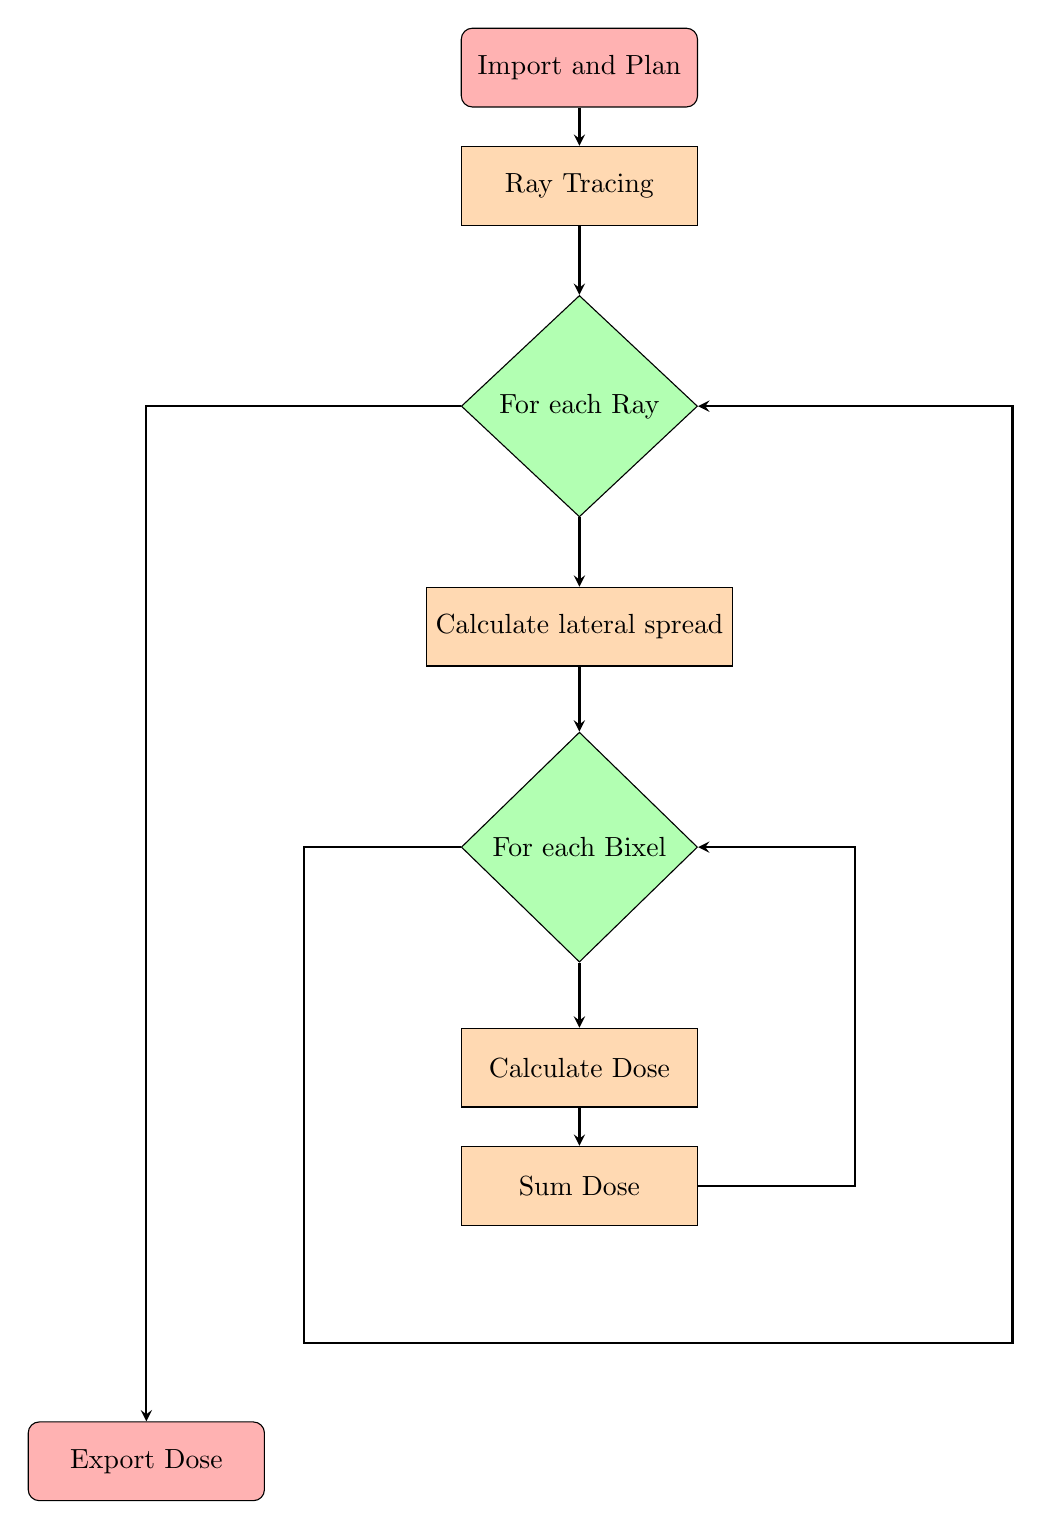
\begin{tikzpicture}[node distance=1.5cm, xshift=5cm]

\node (start) [startstop, xshift=-5cm] {Import and Plan};

\node (rt) [process, below of=start] {Ray Tracing};
\node (loopray) [decision, below of=rt, yshift=-1.3cm] {For each Ray};
\node (geo) [process, below of=loopray, yshift=-1.3cm] {Calculate lateral spread};
\node (loopbixel) [decision, below of=geo, yshift=-1.3cm] {For each Bixel};
\node (calcdose) [process, below of=loopbixel, yshift=-1.3cm] {Calculate Dose};
\node (store) [process, below of=calcdose] {Sum Dose};

\node (end) [startstop, below of=store, xshift=-5.5cm, yshift=-2cm] {Export Dose};

\node[coordinate] (r_store) [right of=store, xshift=2cm] {};
\node[coordinate] (r_loopbixel)   [right of=loopbixel, xshift=2cm] {};
\node[coordinate] (l_loopbixel)   [left of=loopbixel, xshift=-2cm] {};
\node[coordinate] (ls_store)   [left of=store, xshift=-2cm, yshift=-2cm] {};
\node[coordinate] (rs_store)   [right of=store, xshift=4cm, yshift=-2cm] {};
\node[coordinate] (r_loopray)   [right of=loopray, xshift=4cm] {};
\node[coordinate] (l_loopray)   [left of=loopray, xshift=-4cm] {};



\draw [arrow] (start) -- (rt);
\draw [arrow] (rt) -- (loopray);
\draw [arrow] (loopray) -- (geo);
\draw [arrow] (geo) -- (loopbixel);
\draw [arrow] (loopbixel) -- (calcdose);
\draw [arrow] (calcdose) -- (store);
\draw[arrow] (store) -- (r_store) -- node[midway, left]{} (r_loopbixel) -- (loopbixel) ;
\draw[arrow] (loopbixel) -- (l_loopbixel) -- (l_loopbixel) -- (ls_store) -- (rs_store) -- (r_loopray) -- (loopray);
\draw[arrow] (loopray) -- (l_loopray) -- (end);
%\draw [arrow] (loopray) |- (end);

\end{tikzpicture}
\caption{Pencil beam algorithm flowchart. This is repeated for every direction of irradiation}
\label{tikz:pba}
\end{figure}
\newpage

\subsection{Fine Sampling Pencil Beam}
A modified version of pencil beam algorithms consists in the \emph{Fine Sampling}\footnote{Soukup (et al.) \cite{souk:pba}, describes the overall methods behind the Fine Sampling Pencil Beam and shows some of the results}.
The main difference is that fine sampling, as the name suggests, does not calculate the Dose for the whole bixel in one step but divides the bixel in smaller sub-beams and repeats the Dose calculation for all of them. 
\begin{figure}[t]
{\includegraphics[width=.5\textwidth]{Images/FurtherSigmaAnalysis2_01}}
{\includegraphics[width=.5\textwidth]{Images/FurtherSigmaAnalysis2_02}}
\caption{$\gamma$-index value (compared with MC) and maximum percentage error, variating $\sigma_{sub}$, for the inhomogeneous phantom. The red line means the gamma index value of MatRad simulation.}
\label{fig:sigsub}
\end{figure}

The first part of the code is very similar. But before running the loop over the bixels, we need to assign a weight to the sub-components. These are arranged on a square grid at regular distance one to another, covering $3\,\sigma$ of the lateral spread of the beam profile. 
We should have that the gaussian profile of the beam (with standard deviation $\sigma$) and the profile given by the sum of the components (with standard deviation $\sigma_{sub}$) shuold be equal
\[
\frac{1}{\sqrt{2 \pi}\sigma}e^{(x^2+y^2)/2\sigma} = \sum_{i=1}^N \frac{w_i}{\sqrt{2 \pi}\sigma_{sub}}e^{[(x-\mu_{xi})^2+(y-\mu_{yi})^2]/2\sigma_{sub}}
\]
Where $N$ is the number of sub-components, $\mu_{xi}$ and $\mu_{yi}$ are the spacing of the grid and $w_i$ are the weights of each component.
Obviously a component near to the center should give a higher contribute than a component further away and they do not have the same impact on the Dose. So I imposed the weights to be gaussian shaped and I used a function that finds the correct weights, minimizing the square of the difference between the \textbf{suddette} functions.
In formula
\[
\sum^M_{j=1}\, \bigg|\frac{1}{\sqrt{2\pi}\sigma}e^{(x_j^2+y_j^2)/2\sigma}\, - \sum^N_{i=1} \,\frac{W}{\sqrt{2\pi}\Sigma}e^{(x_j^2+y_j^2)/2\Sigma} \,\frac{1}{\sqrt{2\pi}\sigma_{sub}}e^{[(x_j-\mu_{xi})^2+(y_j-\mu_{yi})^2]/2\sigma_{sub}} \bigg|^2
\]
Where $M$ is the number of points on which the minimization run, $W$ and $\Sigma$ are the parameters of the minimization.
The value of $\sigma_{sub}$ has been chosen on the basis of the accuracy of simulations (evaluated with $\gamma$-index test, compared with Monte Carlo simulations) and the maximum error (on the difference between gaussian profile and sum of gaussians). I run simulations on all the configuration, with $\sigma_{sub}/\sigma$ variating from 0.1 to 0.8. I figure \ref{fig:sigsub}, you can see the results for one of the cases. The results are very similar for every phantom and from these we obtained that the most suitable value for our purposes is $\sigma_{sub}/\sigma=0.25$ because it has the highest gamma-index between the values with a error smaller than $1\%$.
\begin{figure}[t]
{\includegraphics[width=.5\textwidth]{Images/gaugrid_2}}
{\includegraphics[width=.5\textwidth]{Images/gausurf_plus}}
\caption{Gaussian lateral profile with highlighted position of the sub-components (left). Gaussian profile of sub-components (right)}
\label{fig:gaugrid}
\end{figure}

%%% adjust sigma figures: -xlabel;  -repeat calculations;  -

%%%% da fare:
%%%%		- ricalcolare gamma index e computation time per numero di sub-components
%%%%		- ricalcolare gamma index e max percentage error per sigma
%%%%		- aggiungere grafici ottenuti
%%%%		- infornare a 180° per un'ora

%%% add sigma further analysis

The other introduction in the code is a function that projects the radiation depth on the central axis of every sub-component. In other words, a new ray tracing for the smaller sub-beams.
Then Radiation depth, used for rescaling of longitudinal distance, is recalculated only for the central axis of the single sub-beam (e.g. the bragg peak is not deformed, it is only scaled on the direction of the beam). I would like to focus the attention of the reader on this point. The sub-component does not take in account the general morphology of the target but only the one corresponding to the voxels crossed by its central axis, in other words, it does not take in account inhomogeneities near the sub-beam axis if they are not \emph{on} the axis. I will show in details this issue in the next chapter. 
In order to compensate this deficiency, a large number of sub-beams should be used. 
As can be easy to forecast, the higher is the number of sub-beams the higher is the accuracy of the simulation. 
The number of sub-components used is $N=324$. This number has been chosen after analysis on computation time, more than accuracy. As one can see from figure \ref{fig:gausn}, the gain in accuracy is almost irrelevant compared with the loss in computation time. For high $N$, the computation has also other problems, such as memory issues because of the huge amount of data in the RAM.
\begin{figure}[t]
{\includegraphics[width=.5\textwidth]{Images/gamman}}
{\includegraphics[width=.5\textwidth]{Images/timen}}
\caption{Gamma index (left) and time consumption (right) as function of $n$. The value $n$ on the $x$-axis is related with the number of compontents as $N=(2n+2)^2$}
\label{fig:gausn}
\end{figure}

The new flowchart of the model (\ref{tikz:fs}) is very similar to the previous one but with one more loop.
%%% add figures:
%%%		- sub-gaussians
%%%		- grid
Apart for the weights, there is a function that allows the projection .........


%\begin{figure}[!h]
%\centering
%\begin{tikzpicture}[node distance=1.5cm, xshift=5cm]
%
%\node (start) [startstop, xshift=-5cm] {Import and Plan};
%
%\node (rt) [process, below of=start] {Ray Tracing};
%\node (loopray) [decision, below of=rt, yshift=-1.3cm] {For every Ray};
%\node (geo) [process, below of=loopray, yshift=-1.3cm] {Calc lateral distances};
%\node (loopbixel) [decision, below of=geo, yshift=-1.3cm] {For every Bixel};
%\node (calcdose) [process, below of=loopbixel, yshift=-1.3cm] {Calculate Dose};
%\node (store) [process, below of=calcdose] {Store Dose};
%
%\node (end) [startstop, below of=store, xshift=-5.5cm, yshift=-2cm] {Export Dose};
%
%\node[coordinate] (r_store) [right of=store, xshift=2cm] {};
%\node[coordinate] (r_loopbixel)   [right of=loopbixel, xshift=2cm] {};
%\node[coordinate] (l_loopbixel)   [left of=loopbixel, xshift=-2cm] {};
%\node[coordinate] (ls_store)   [left of=store, xshift=-2cm, yshift=-2cm] {};
%\node[coordinate] (rs_store)   [right of=store, xshift=4cm, yshift=-2cm] {};
%\node[coordinate] (r_loopray)   [right of=loopray, xshift=4cm] {};
%\node[coordinate] (l_loopray)   [left of=loopray, xshift=-4cm] {};
%
%
%
%\draw [arrow] (start) -- (rt);
%\draw [arrow] (rt) -- (loopray);
%\draw [arrow] (loopray) -- (geo);
%\draw [arrow] (geo) -- (loopbixel);
%\draw [arrow] (loopbixel) -- (calcdose);
%\draw [arrow] (calcdose) -- (store);
%\draw[->] (store) -- (r_store) -- node[midway, left]{} (r_loopbixel) -- (loopbixel) ;
%\draw[->] (loopbixel) -- (l_loopbixel) -- (l_loopbixel) -- (ls_store) -- (rs_store) -- (r_loopray) -- (loopray);
%\draw[->] (loopray) -- (l_loopray) -- (end);
%%\draw [arrow] (loopray) |- (end);
%
%\end{tikzpicture}
%\caption{Pencil beam algorithm flowchart}
%\label{tikz:pba}
%\end{figure}
%\newpage




%b\footnote{Siemens link to Syngo page: \url{https://www.healthcare.siemens.it/medical-imaging-it}}

\section{Phantom Data}
\begin{figure}[h]
{\includegraphics[width=0.55\textwidth]{Images/PTW_31015}}
{\includegraphics[width=0.45\textwidth]{Images/PTW_31015spec}}
\caption{Single PTW-31015 ionization chamber, on the right (left picture), and precise description of its dimensions (right picture)}
\label{fig:31015}
\end{figure}
%troppi rimandi ad altre fonti......spiega un po' di pi�!
We compared our data with a set of measurements done at HIT center. The target consists of a plexiglass box filled with water with a detector inside. The detector is composed by 24 ionization chambers models \emph{PTW-31015}\footnote{A complete set of specifications can be found at \url{https://www.rpdinc.com/ptw-31015-003-cc-pinpoint-chamber-976.html}} produced by PTW-Freiburg\footnote{\url{http://www.ptw.de/home_start.html?&no_cache=1}}. The ionization chambers have a cylindrical shape with vented sensitive volumes of $30\,mm^3$ ($1.45\,mm$, length $5\,mm$) and $2.9\,mm$ in external diameter (figure \ref{fig:31015}).
%% The productor declares a nominal response of $800\,pC/Gy$. (\textbf{from this i should find the error on the measurement but i miss some data})
The chambers are arranged in 6 lines on 3 levels, inside a plexiglass support that allows to immerse the chambers directly inside the water. In figure \ref{fig:24cham} is shown the set up of the detector.
The colleagues of the Hadron therapy center collected data from measurements in nine different positions where the whole detector was moved inside the volume and across the surface of a cubic target area. More about this measurements will be tell in the next chapter.

\begin{figure}[h]
{\includegraphics[width=\textwidth]{Images/Siemens24chambers}}
\caption{Photographs of the complete mounted detector from different points of view}
\label{fig:24cham}
\end{figure}
\subsection{Water boxes and simple configurations}
\subsection{Double Wedge}
The Double Wedges is a particular kind of phantom built from HIT colleagues with the aim of trying the effects of the treatment through a surface that has a considerable slope at the entrance surface. %??????????????????????ci sono i fantasmi OoO
\subsection{Alderson phantom}
\subsection{HU and Stopping Power}

\section{Analysis techniques}
\subsection{Dose Profiles}
\subsection{Dose difference Maps}
MatRad was initially thought as a dose calculation software based on the same concept as the Siemens product. The result of every simulation is a cube of $512\times512\times39$ voxels, that is the same dimension as the CT-cube. When I refer to the percentage difference between two cubes, I mean the difference in percentage made point-by-point from one voxel of the first cube to the respective one on the second cube. %???????metti o un disegno o qualche formula o aggiungi qualcosa che faccia capire meglio
\subsection{Gamma Index}
The peculiar attribute of the dose deposition simulations is to have large flat or low-gradient zones, usually inside and outside the target area and very-high-gradient zones in the region surrounding it (or tumor in real cases).
The mathematical difference between two datasets will not give us a full and exhaustive comparison because it could highlights an area of significant disagreement near high-gradient regions and a more quantitative assessment may be needed for final system approval.   
\begin{figure}[b!]
\includegraphics[width=\textwidth]{Images/Images/highGradientExample.png}
\caption{Example of the difference (right) between two identical curves with high-gradient(left)}
\label{fig:highgrad}
\end{figure}
For example: if one compares two sets of identical data but shifted of a fraction of the millimeter, as in figure~\ref{fig:highgrad}, the difference will have a very pronounced peak that could be considered out of our tolerance range for the dose axis but inside our acceptance level for the distance.
In order to avoid this issue, I used the method shown in Low \emph{et al.} \cite{low:gamma} or else the \emph{gamma-index test} that uses a distance-to-agreement (DTA) distribution to determine the acceptability of the dose calculation. The DTA is the distance between a measured data point and the nearest point in the calculated dose distribution that exhibits the same dose. Each measured point is evaluated to determine if both dose difference and DTA exceed the selected respective tolerances. Points that fail both criteria are identified on a composite distribution. This is an extension of the isodose comparison tool that simultaneously incorporates the dose and the distance criteria and provides a numerical quantity index (further called $gamma$-index) that serves as a measure of disagreement in the regions that fail the acceptance criteria and indicates the calculation quality in the regions that pass. A further and Mathematical explanation is given in Appendix A.
%riscrivi meglio la prima parte non ho capito una \hbar

\subsubsection{Interpolation}


\chapter{Results} %%%%%%%%%%%%%%%%%%%%%%%%%%%%%%%%%%%%%%%%%%%%%%%%%%%%%%%%%%%%%%%%%
\label{chap:res}



In order to give an accurate and full comparison between the algorithms that we considered, I will proceed by several steps, starting from the simplest example towards more complicated and realistic treatment fields.




\section{Elementary Pencil Beams}
The basic starting point for a comparison between similar methods is to actually confirm that they are similar in very simple cases. Only after one is allowed to proceed and analyse more sophisticated problems. 

\subsubsection{Water Box}
The easiest case that we can put our hands on is the full Water Box. Nothing more than a fully symmetrical cubic box made of water.
The dose simulations gave us the result in figure\ref{fig:WB1}, where the Isocenter slice of the dose cubes is plotted.
\begin{figure}[!ht]
\centering
\subfloat[][\emph{MatRad}]
{\includegraphics[width=.31\textwidth]{Images/Images_homog_phantom/mR_FSBvsMC_pub_homog_notitle_01.png}}
\subfloat[][\emph{Fine Sampling}]
{\includegraphics[width=.31\textwidth]{Images/Images_homog_phantom/mR_FSBvsMC_pub_homog_notitle_02.png}}
\subfloat[][\emph{Monte Carlo}]
{\includegraphics[width=.31\textwidth]{Images/Images_homog_phantom/mR_FSBvsMC_pub_homog_notitle_03.png}}
\caption{Dose deposition in water box}
\label{fig:WB1}
\end{figure}


The full agreement of these data sets can be confirmed by the percentage difference map and the $\gamma$-index test. Figure \ref{fig:WB1gam} shows excellent results.
\begin{figure}[!ht]
\centering
\subfloat[][\emph{Percentage\\ difference}]
{\includegraphics[width=.25\textwidth]{Images/Images_homog_phantom/mR_FSBvsMC_pub_homog_notitle_04n.png}} 
\subfloat[][\emph{$\gamma$-index \\ $99.92\%$ [$1\%$ $1mm$]}]
{\includegraphics[width=.25\textwidth]{Images/Images_homog_phantom/mR_FSBvsMC_pub_homog_notitle_05n.png}}
\subfloat[][\emph{Percentage\\ difference}]
{\includegraphics[width=.25\textwidth]{Images/Images_homog_phantom/mR_FSBvsMC_pub_homog_notitle_06n.png}} 
\subfloat[][\emph{$\gamma$-index \\ $99.92\%$ [$1\%$ $1mm$]}]
{\includegraphics[width=.25\textwidth]{Images/Images_homog_phantom/mR_FSBvsMC_pub_homog_notitle_07n.png}} 
\caption{Comparison between MatRad and Monte Carlo (left), Fine Sampling and Monte Carlo (right) in water box}
\label{fig:WB1gam}
\end{figure}

One easy notable thing is the light shift in the Bragg peak position. From the central profile (in figure \ref{fig:WB1prof}), we measured a shift of $0.13\pm0.10\,mm$ and $0.12\pm0.10\,mm$ in the direction of the beam, for Fine Sampling and MatRad respectively. In figure \ref{fig:WB1profz} there is a zoomed image of both these profiles.
The measured integral dose is $103.3\,cGy$ for MatRad $103.0\,cGy$ for Fine Sampling and $103.7\pm1.0\,cGy$ for Monte Carlo simulations.\\
\\

\begin{figure}[!ht]
\centering
\subfloat[][\emph{Central Dose profile}]
{\includegraphics[width=.45\textwidth]{Images/Images_homog_phantom/CP_wb_zoom.png}} 
\subfloat[][\emph{Integrated Depth Dose profile}]
{\includegraphics[width=.45\textwidth]{Images/Images_homog_phantom/IDD_wb_zoom.png}} \\
\subfloat[][\emph{Phantom surface entering profile}]
{\includegraphics[width=.45\textwidth]{Images/Images_homog_phantom/mR_FSBvsMC_pub_homog_notitle_10.png}} 
\subfloat[][\emph{Peak profile}]
{\includegraphics[width=.45\textwidth]{Images/Images_homog_phantom/mR_FSBvsMC_pub_homog_notitle_11.png}}
\caption{Profiles in water box simulation}
\label{fig:WB1prof}
\end{figure}

%\begin{figure}[!ht]
%\centering
%\subfloat[][\emph{Central Dose profile}]
%{\includegraphics[width=.45\textwidth]{Images/Images_homog_phantom/CP_wb_zoom.png}} 
%\subfloat[][\emph{Integrated Depth Dose profile}]
%{\includegraphics[width=.45\textwidth]{Images/Images_homog_phantom/IDD_wb_zoom.png}}
%\caption{Profiles in water box simulation, zoomed}
%\label{fig:WB1profz}
%\end{figure}

The next case will be a beam entering the phantom with a $30^\circ$ angle. This example is important to understand the basic differences between MatRad and Fine Sampling algorithms. As you can see from figure \ref{fig:WB2}, the shape of these dose depositions appears different compared with the Monte Carlo simulation. The reason why they behave in this way comes from the evaluation of the radiation depth. MatRad, as a software based on \emph{Ray Casting}, calculates the radiation depth for every possible particle direction and adjusts the precomputed bragg peak in water to the aforementioned radiation depth. Fine sampling instead divides the incoming particle fluence in several sub-beams and their radiation depth is evaluated singularly and only on the central axis of the sub-sample giving a better sensitivity to the morphology of the target but a bad response on to small inhomogeneities inside the tissue.
This is the reason for a considerable shift of the Bragg Peak in the central and lateral dose profile of the peak, shown in figure \ref{fig:WB2prof}. I calculated the shift and I got $0.4\pm0.3\,mm$ for the Fine Sampling algorithm and $0.7\pm0.4\,mm$ for the MatRad algorithm. This can be considered a great result given the $3mm$ resolution of the CT data.
The total Dose deposited is $811.9$, $810.2$ and $813.2\pm8.1\,cGy$ for MatRad, Fine Sampling and Monte Carlo respectively.\\
\\

\begin{figure}[!t]
\centering
\subfloat[][\emph{MatRad}]
{\includegraphics[width=.31\textwidth]{Images/Images_homog_phantom/mR_FSBvsMC_pub_homog_notitle_12.png}}\quad
\subfloat[][\emph{Fine Sampling}]
{\includegraphics[width=.31\textwidth]{Images/Images_homog_phantom/mR_FSBvsMC_pub_homog_notitle_13.png}}\quad
\subfloat[][\emph{Monte Carlo}]
{\includegraphics[width=.31\textwidth]{Images/Images_homog_phantom/mR_FSBvsMC_pub_homog_notitle_14.png}}\quad
\caption{Dose deposition in water box, $30^\circ$ degree entering beam}
\label{fig:WB2}
\end{figure}

\begin{figure}[]
\centering
\subfloat[][\emph{Percentage difference and\\ $\gamma$-index  $98.77\%$ [$3\%$ $3mm$]}]
{\includegraphics[width=.45\textwidth]{Images/Images_homog_phantom/mR_FSBvsMC_pub_homog_30g_mR.png}} 
\subfloat[][\emph{Percentage difference and \\$\gamma$-index  $96.86\%$ [$3\%$ $3mm$]}]
{\includegraphics[width=.45\textwidth]{Images/Images_homog_phantom/mR_FSBvsMC_pub_homog_30g_FS.png}} 
\caption{Comparison between MatRad and Monte Carlo (left), Fine Sampling and Monte Carlo (right) in water box, $30^\circ$ degree entering beam}
\label{fig:WB2gam}
\end{figure}

\begin{figure}[!ht]
\centering
\subfloat[][\emph{Central Dose profile}]
{\includegraphics[width=.45\textwidth]{Images/Images_homog_phantom/mR_FSBvsMC_pub_homog_notitle_19.png}} 
\subfloat[][\emph{Peak profile}]
{\includegraphics[width=.45\textwidth]{Images/Images_homog_phantom/mR_FSBvsMC_pub_homog_notitle_22.png}}
\caption{Profiles in water box simulation, $30^\circ$ degree entering beam}
\label{fig:WB2prof}
\end{figure}

\begin{figure}[!t]
\centering
\subfloat[][\emph{MatRad}]
{\includegraphics[width=.31\textwidth]{Images/Images_homog_phantom/mR_FSBvsMC_pub_homog_notitle_23.png}}\quad
\subfloat[][\emph{Fine Sampling}]
{\includegraphics[width=.31\textwidth]{Images/Images_homog_phantom/mR_FSBvsMC_pub_homog_notitle_24.png}}\quad
\subfloat[][\emph{Monte Carlo}]
{\includegraphics[width=.31\textwidth]{Images/Images_homog_phantom/mR_FSBvsMC_pub_homog_notitle_25.png}}\quad
\caption{Dose deposition in water box, $45^\circ$ degree entering beam}
\label{fig:WB3}
\end{figure}

\begin{figure}[]
\centering
\subfloat[][\emph{Percentage difference and\\ $\gamma$-index  $96.62\%$ [$3\%$ $3mm$]}]
{\includegraphics[width=.45\textwidth]{Images/Images_homog_phantom/mR_FSBvsMC_pub_homog_45g_mR.png}} 
\subfloat[][\emph{Percentage difference and \\$\gamma$-index  $100\%$ [$3\%$ $3mm$]}]
{\includegraphics[width=.45\textwidth]{Images/Images_homog_phantom/mR_FSBvsMC_pub_homog_45g_FS.png}} 
\caption{Comparison between MatRad and Monte Carlo (upper graphics), Fine Sampling and Monte Carlo (lower graphics) in water box, $45^\circ$ degree entering beam}
\label{fig:WB3gam}
\end{figure}

\begin{figure}[!ht]
\centering
\subfloat[][\emph{Central Dose profile}]
{\includegraphics[width=.45\textwidth]{Images/Images_homog_phantom/mR_FSBvsMC_pub_homog_notitle_30.png}} 
\subfloat[][\emph{Integrated Depth Dose profile}]
{\includegraphics[width=.45\textwidth]{Images/Images_homog_phantom/mR_FSBvsMC_pub_homog_notitle_31.png}} \\
\subfloat[][\emph{Phantom surface entering profile}]
{\includegraphics[width=.45\textwidth]{Images/Images_homog_phantom/mR_FSBvsMC_pub_homog_notitle_32.png}} 
\subfloat[][\emph{Peak profile}]
{\includegraphics[width=.45\textwidth]{Images/Images_homog_phantom/mR_FSBvsMC_pub_homog_notitle_33.png}}
\caption{Profiles in water box simulation, $45^\circ$ degree entering beam}
\label{fig:WB3prof}
\end{figure}

As last but not less interesting is the case of the $45^\circ$-degrees-entering-beam. This shows us, in a more explicit form, the issue of Ray-Casting-algorithms treating surfaces with particular shapes. In figure \ref{fig:WB3}, the first thing we can notice is the artifice in MatRad simulation that reproduces the angle shape of the CT surface in the dose deposition. This is clearly wrong, even if the Monte Carlo simulation outlines the same behaviour in a smoother way. Fine sampling produces a wrong interpretation caused by the weights assigned to the sub-beams. In other words, it gives to the central beam almost twice the weight of the nearest lateral sub-beams and almost 20 times more compared to the most lateral ones.
Even though this little issue does not compromise the accuracy of the Fine Sampling simulation, as attested from the comparison tests in figure \ref{fig:WB3gam} and figure \ref{fig:WB3prof}. From this last figures, I measured a shift of $0.3\pm0.3\,mm$ for the Fine Sampling and $0.9\pm0.7\,mm$ for MatRad in the beam direction, and an integrated Dose of $946.8$, $940.3$ and $951.5\pm10.7\,cGy$ for MatRad, the Fine Sampling and the Monte Carlo respectively.

\subsubsection{Inhomogeneous Water Box}
\begin{figure}[!t] 
%%%%%% replace figures with correct ones %%%%%%%
\centering
\subfloat[][\emph{MatRad}]
{\includegraphics[width=.31\textwidth]{Images/Images_homog_phantom/mR_FSBvsMC_pub_homog_notitle_01.png}}\quad
\subfloat[][\emph{Fine Sampling}]
{\includegraphics[width=.31\textwidth]{Images/Images_homog_phantom/mR_FSBvsMC_pub_homog_notitle_02.png}}\\
\subfloat[][\emph{Monte Carlo}]
{\includegraphics[width=.31\textwidth]{Images/Images_homog_phantom/mR_FSBvsMC_pub_homog_notitle_03.png}}\quad
\subfloat[][\emph{Fine Sampling Plus}]
{\includegraphics[width=.31\textwidth]{Images/Images_homog_phantom/mR_FSBvsMC_pub_homog_notitle_02.png}}
\caption{Dose deposition in inhomogeneous water box}
\label{fig:HWB1}
\end{figure}

This water box consists of a cube divided in two parts along the beam direction, one filled with water and the other one with a material with a slightly smaller electron density.
The aim is to show how Ray Casting algorithms sees this kind of phantoms.
Ray casting gives back a dose with a clear step in it, caused by the same mechanism discussed before. The comparison with Monte Carlo simulation gives a surprising far better result than Fine Sampling, i.e. a $97.59\%$ of passing points with a [$3\%$ $3mm$] criterion against the $92.69\%$ of the Fine Sampling, in the same conditions. This algorithm has a disadvantage in this experiment, that is the high weight of the central beam. The method that I adopted in order to try to solve this issue is using a Fine Sampling model with a greater number of sub-beams, in order to make them narrower and with a more balanced weigh. I chose to bring the number of beams from 19 to 729 and, as you can see from the dose deposition in figure \ref{fig:HWB1} and from comparisons in figure \ref{fig:HWB1gam}, the so called Fine Sampling Plus  improves the accuracy over MatRad level.


\begin{figure}[!ht]
%%%%%% replace figures with correct ones %%%%%%%
\centering
\subfloat[][\emph{Percentage difference}]
{\includegraphics[width=.45\textwidth]{Images/Images_homog_phantom/mR_FSBvsMC_pub_homog_notitle_04.png}} 
\subfloat[][\emph{$\gamma$-index  $97.59\%$ [$3\%$ $3mm$]}]
{\includegraphics[width=.45\textwidth]{Images/Images_homog_phantom/mR_FSBvsMC_pub_homog_notitle_05.png}} \\
\subfloat[][\emph{Percentage difference}]
{\includegraphics[width=.45\textwidth]{Images/Images_homog_phantom/mR_FSBvsMC_pub_homog_notitle_06.png}} 
\subfloat[][\emph{$\gamma$-index  $97.91\%$ [$3\%$ $3mm$]}]
{\includegraphics[width=.45\textwidth]{Images/Images_homog_phantom/mR_FSBvsMC_pub_homog_notitle_07.png}} 
\caption{Comparison between MatRad and Monte Carlo (upper graphics), Fine Sampling Plus and Monte Carlo (lower graphics) in inhomogeneous water box}
\label{fig:HWB1gam}
\end{figure}





\newpage

\section{Spread-Out Bragg Peak}

\section{Realistic Treatment Fields}
\subsection{Double Wedge}
\subsubsection{Full Field}

In this section, I expound the predictions made with MatRad and Syngo and I compare them also by using the $\gamma$-index test. The figures shown are slices of a sagittal plane of the phantom passing through the isocenter of the CT-cube
\begin{figure}[!ht]
\centering
\subfloat[][\emph{Syngo}]
{\includegraphics[width=.45\textwidth]{Images/Images/epub_comparison2_01.png}} \quad
\subfloat[][\emph{MatRad}]
{\includegraphics[width=.45\textwidth]{Images/Images/epub_comparison2_02.png}} \quad
\caption{Simulated Double Wedges Dose deposition}
\label{fig:SyngoMat}
\end{figure}

a

\begin{figure}[t]
\centering
\subfloat[][\emph{Percentage Dose Difference}]
{\includegraphics[width=.65\textwidth]{Images/Images/epub_comparison2_03.png}} \\
\subfloat[][\emph{Gamma index test with parameters 1\% - 1$mm$}]
{\includegraphics[width=.65\textwidth]{Images/Images/epub_comparison2_04.png}} \\
\subfloat[][\emph{Gamma index test with parameters 2\% - 2$mm$}]
{\includegraphics[width=.65\textwidth]{Images/Images/epub_comparison2_05.png}} \quad
\caption{Comparison between MatRad and Syngo}
\label{fig:SyngoMat2}
\end{figure}

\subsubsection{Measurements}
The last step of my work is to check the compatibility of our prediction with the real measurements. These are our gold standard and the final test that every software has to overcome to be consider a good predictor.

As I said in Chapter 2, the detector inside Double Wedges Phantom has been placed in 9 different positions and, for each of them, I have the dose value measured in every chamber and that one predicted by Syngo. In this case, the simulation with Syngo has been made in two different ways. The first simulates the whole proton beam and the dose deposition inside the CT-cube (it works in the same way as MatRad does), then from this cube the values of dose in the areas covered by every single chamber are extracted. The second one, referred as Syngo, evaluates the dose directly inside the area covered by every single ionization chamber, this causes a slightly difference between them.

In the following pages, I will show a series of images where it is shown a slice of the dose cube evaluated with MatRad and the projection of the position of the 24 chambers, all in CT resolution. Associated to this set of images, there is a graph that reports the actual value in $cGy$ of the ionization chambers for measurements and simulations.
\newpage
\begin{figure}[h!]
\centering
\subfloat[][\emph{Sagittal plane}]
{\includegraphics[width=.65\textwidth]{Images/Images/Meas_MR_comparison_01.png}} \quad
\subfloat[][\emph{Coronal plane}]
{\includegraphics[width=.65\textwidth]{Images/Images/Meas_MR_comparison_02.png}} \\
\subfloat[][\emph{Ionization chambers values}]
{\includegraphics[width=.65\textwidth]{Images/Images/Meas_MR_comparison_03.png}} \quad
\caption{Results, geometry and comparison from configuration 1}
\label{fig:pos1}
\end{figure}

\newpage
\begin{figure}[h!]
\centering
\subfloat[][\emph{Sagittal plane}]
{\includegraphics[width=.45\textwidth]{Images/Images/Meas_MR_comparison_01.png}} \quad
\subfloat[][\emph{Coronal plane}]
{\includegraphics[width=.45\textwidth]{Images/Images/Meas_MR_comparison_02.png}} \\
\subfloat[][\emph{Ionization chambers values}]
{\includegraphics[width=.45\textwidth]{Images/Images/Meas_MR_comparison_03.png}} \quad
\caption{Results, geometry and comparison from configuration 2}
\label{fig:pos2}
\end{figure}

\subsection{Alderson phantom}

\section{Overview} % Mean tables


\chapter{Discussion} %%%%%%%%%%%%%%%%%%%%%%%%%%%%%%%%%%%%%%%%%%%%%%%%%%%%%%%%%%%%%%

\section{Summary}
\section{Interpretation}
\section{Other Published Data}

\chapter{Conclusions} %%%%%%%%%%%%%%%%%%%%%%%%%%%%%%%%%%%%%%%%%%%%%%%%%%%%%%%%%%%%%

\appendix
\chapter{$\gamma$-index test}

\tableofcontents
\listoffigures
\listoftables

\begin{thebibliography}{99}

\bibitem{bang:apm}
Bangert M., Hennig P., Oelfke U. -
\emph{Analytical probabilistic modeling for radiation therapy treatment planning} - 
Phys. Med. Biol. 58 5401–5419 (2013)

\bibitem{boeh:fluka}
Böhlen T.T., Cerutti F., Chin M.P.W., Fassò A., Ferrari  A., Ortega P.G., Mairani A., Sala P.R., Smirnov G. and Vlachoudis V. -
\emph{The FLUKA Code: Developments and Challenges for High Energy and Medical Applications} -
Nuclear Data Sheets 120, 211-214 (2014) 

\bibitem{bort:bragg}
Bortfeld T. -
\emph{An analytical approximation of the Bragg curve for therapeutic proton beams} -
Med. Phys. 24, 2024-33 (1997)

\bibitem{bort:SOBP}
Bortfeld T. and Schlegel W. -
\emph{An analytic approximation of depth–dose distributions for therapeutic proton beams} -
Phys. Med. Biol. 41, 1331–9 (1996)

\bibitem{ferr:fluka}
Ferrari A., Sala P.R., Fassò A. and Ranft J. -
\emph{FLUKA: a multi-particle transport code} -
CERN-2005-10, INFN/TC\_05/11, SLAC-R-773 (2005)

\bibitem{high:mcs}
Highland V.L. -
\emph{Some practical remarks on multiple scattering} -
Nucl. Instr. Meth. Phys. Res. 129, 497–499 (1975)

\bibitem{jett:SOBP}
Jette D. and Chen W. - 
\emph{Creating a spread-out Bragg peak in proton beams} -
Phys. Med. Biol. 56, N131–N138 (2011)

\bibitem{Kram:track}
Krämer M. - 
\emph{Calculations of heavy-ion track structure} - 
Nucl. Instr. Meth. Phys. Res. B 105, 14–20 (1995)

\bibitem{low:gamma}
Low D. A., Harms W. B., Mutic S. and Purdy J. A. -
\emph{A technique for the quantitative evaluation of dose distributions} -
Med. Phys. 25, 5 (1998)

\bibitem{mol:mcs}
Molière G. -
\emph{Theorie der Streuung schneller geladener Teilchen II, Mehrfach- und Vielfachstreuung} - 
Z. Naturforsch. 3a, 78–97 (1948)

\bibitem{par:latspr}
Parodi K., Mairani A., Sommerer F. -
\emph{Monte Carlo-based parametrization of the lateral dose spread for clinical treatment planning of scanned proton and carbon ion beams} -
Journal of Radiation Research 54, i91–i96 (2013)

\bibitem{schaf:pba}
Schaffner B., Pedroni E. and Lomax A. -
\emph{Dose calculation models for proton treatment planning using a dynamic beam delivery system: an attempt to include density heterogeneity effects in the analytical dose calculation} - 
Phys. Med. Biol. 44, 27–41 (1999)

\bibitem{schn:mcs}
Schneider U., Besserer J., Pemler P. - 
\emph{On small angle multiple Coulomb scattering of protons in the Gaussian approximation} - 
Z. Med. Phys. 11,  110- 118 (2001)

\bibitem{serb:nucRea}
Serber R. - 
\emph{Nuclear reactions at high energies} -
Phys. Rev. 72(11), 1114–1115 (1947)

\bibitem{souk:pba}
Soukup M., Fippel M. and Alber M. -
\emph{A pencil beam algorithm for intensity modulated proton therapy derived from Monte Carlo simulations} -
Phys. Med. Biol. 50, 5089–5104 (2005)

\bibitem{weyr:rbe}
Weyrather W.K., Ritter S., Scholz M., Kraft G. - 
\emph{RBE for carbon track-segment irradiation in cell lines of differing repair} -
capacity. Int. J. Radiat. Biol. 75, 1357–1364 (1999)



%% aggiungere history of hadrontherapy dell'amaldi e del degiovanni


\end{thebibliography}


%%%%%%%%%%%%%%%%%%%%%%%%%%%%%%%%%%%%% TO DO Section %%%%%%%%%%%%%%%%%%%%%%%%%%%%%%%%%%%%
% 1) Change the figures with the correct ones and change the gamma index pass rate.

% 2) Add some new images for the Double Wedges phantom.

% 3) 


\end{document}
